\documentclass{article}
\usepackage[utf8]{inputenc}
\usepackage[english]{babel}

\title{Red Black Trees}
\author{Manuel Serna-Aguilera}
\date{}
\setlength{\parindent}{0pt}

\usepackage{natbib}
\usepackage{graphicx}
\usepackage{amsmath}
\usepackage{clrscode3e}
\usepackage{amsthm}

\begin{document}

\maketitle

While bst's are nice and all, they may end up horribly balanced to the point where operations' run times are like that of a linked list. Red-black trees attempt to balance the tree so that operations take $O(\log_2{n})$ time.
\\ \\
A red-black tree is a binary search tree with one extra bit of storage--its color, which can be either be red or black. Now, each node contains the main attributes: $\id{color}$, $\id{key}$, $\id{left}$, $\id{right}$, and $\id{p}$, with satellite data.

\section*{Properties}
A red-black tree is a binary search tree that satisfies the following red-black properties:
\begin{enumerate}
    \item Every node is either red or black.
    \item The root is black.
    \item Every leaf is black (the $\const{nil}$ leaves).
    \item If a node is red, then both of its children are black.
    \item For each node, all simple paths from the node to descendant leaves contain the same number of black nodes (all paths from the root must contain the same number of black nodes).
\end{enumerate}
Of course, we tack on the regular bst properties.
\\ \\
All leaf nodes have two children, they are $\const{nil}$ nodes, which are black. In terms of pointers, we can have all the children pointers of the leaf nodes point to a single special node called $\attrib{T}{nil}$ and have its color be black.
\\ \\
\textbf{Black height}: we call the number of black nodes on any simple path from, but \textit{not} including, a node $x$ down to a leaf the black height of a node, denoted $bh(x)$. The $\textbf{\emph{black-height}}$ of a red-black tree is the black height of its root.

\newtheorem*{lemma}{Lemma}

\begin{lemma}
A red-black tree with $n$ internal nodes has height at most $2 \cdot \log_2{(n+1)}$.
\end{lemma}

\newpage

% figure 13.1
\begin{figure}[!ht]
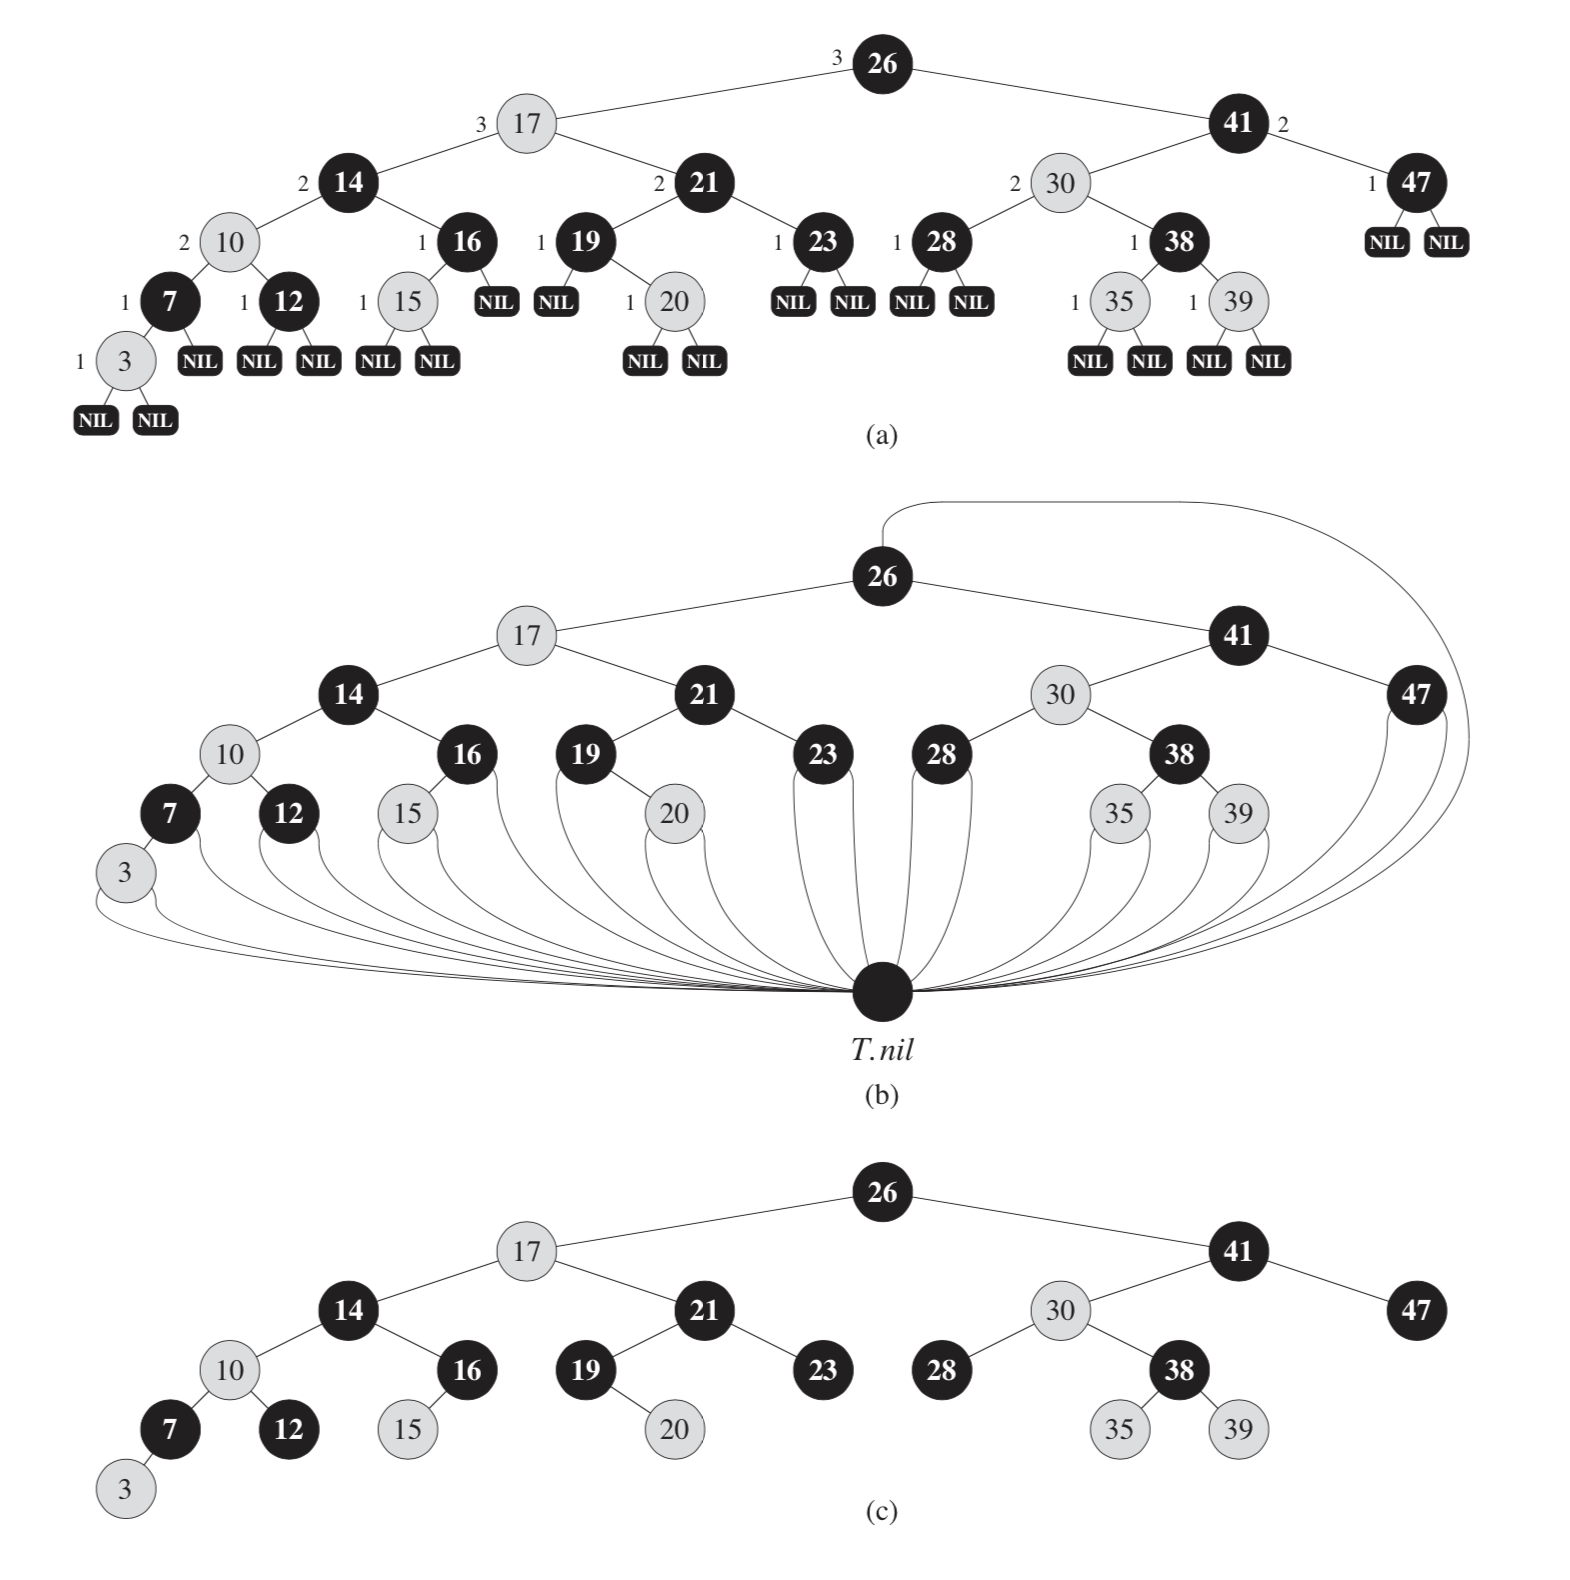
\includegraphics[scale=0.55]{rbt1}
\caption{
    A red-black tree from the book, red nodes are shaded while black nodes are darkened. Notice all the red-black properties apply to this tree.
    \textbf{(a)} Each node is shown with its black height, while also showing all the $\const{nil}$ children, recall they must all be black. 
    \textbf{(b)} Simplifies this view to have all pointers refer to a single node called $\attrib{T}{nil}$.
    \textbf{(c)} What the book will draw to avoid having to draw all the lines and $\attrib{T}{nil}$.
}
\label{fig: rbt1}
\end{figure}

\section*{Rotations}
When we insert or delete nodes to/from a red-black tree, the red-black properties may be violated, and we may have to recolor nodes and change the pointer structure. We change the \textit{pointer structure} through rotation, which is a subroutine that move two nodes and their subtrees around. Note that colors are not changed in the procedure.

% figure 13.2
\begin{figure}[!ht]
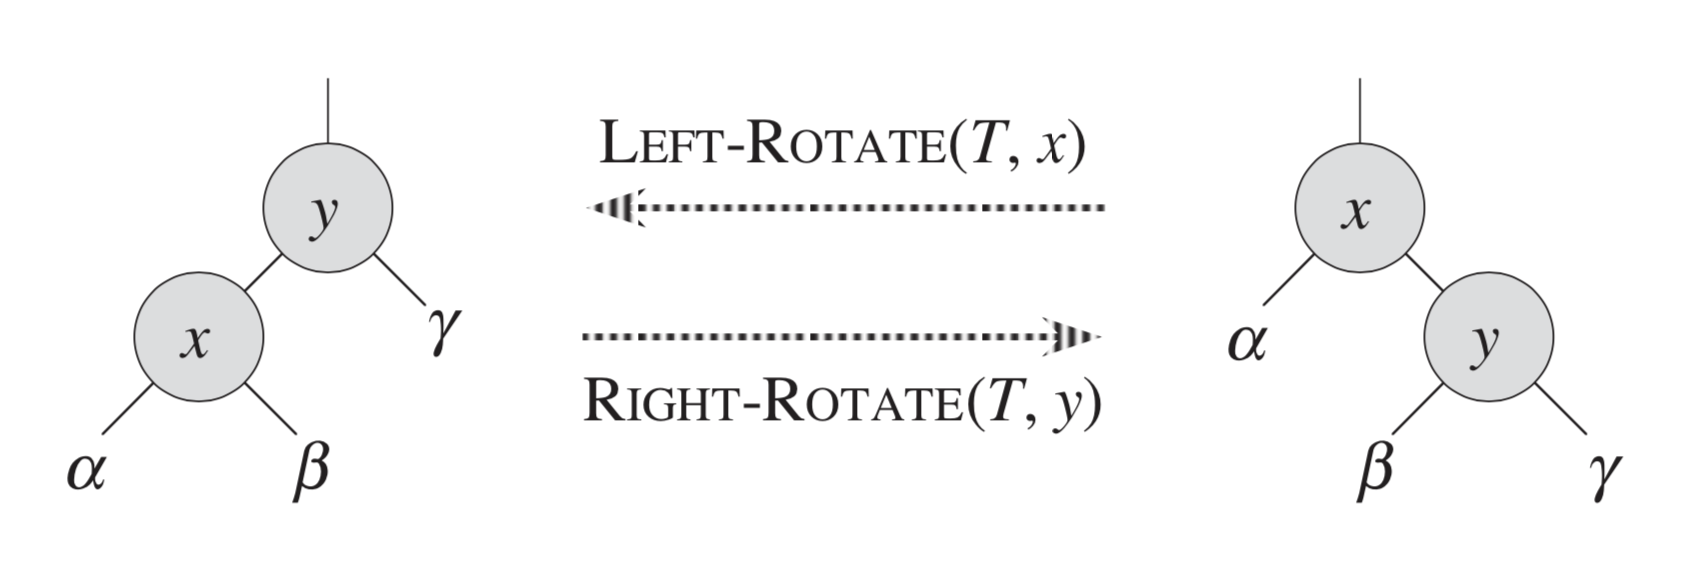
\includegraphics[scale=0.4]{rbt_rotate}
\caption{
    The rotation operations on a binary search tree.
}
\label{fig: rbt2}
\end{figure}

For left rotate on $x$, we rotate around the link between $x$ and its right non-nil child $y$. First we disconnect $x$ and $y$ so $y$ does not reference $x$. Then we move the subtree $\beta$ from being $y$'s left subtree to being $x$'s right subtree (this is the only subtree that ``jumps'' nodes). Next, have $\attrib{y}{p}$ point to $x$'s parent, while making $x$'s parent $y$. We then make $\attrib{y}{left}$ $x$. The process is symmetrical for a right rotate, I have both procedures below.

%--------------------------------------------
% left rotate
%--------------------------------------------
\begin{codebox}
\Procname{$\proc{left-rotate}(T, x)$}
\li $y \gets{\attrib{x}{right}}$ \Comment set y
\li $\attrib{x}{right} \gets{\attrib{y}{left}}$ \Comment turn $y$'s left subtree into $x$'s right subtree
\li \If $\attrib{y}{left} \neq \attrib{T}{nil}$
\li \Then
        $\attrib{y}{\attrib{left}{p}} \gets{x}$
    \End
\li $\attrib{y}{p} \gets{\attrib{x}{p}}$ \Comment link $x$'s parent to $y$
\li \If $\attrib{x}{p} \isequal \attrib{T}{nil}$
\li \Then
        $\attrib{T}{root} \gets{y}$
\li \ElseIf $x \isequal \attrib{x}{\attrib{p}{left}}$
\li \Then
        $\attrib{x}{\attrib{p}{left}} \gets{y}$
\li \Else
\li     $\attrib{x}{\attrib{p}{right}} \gets{y}$
    \End
\li $\attrib{y}{left} \gets{x}$ \Comment put $x$ on $y$'s left
\li $\attrib{x}{p} \gets{y}$
\end{codebox}

%--------------------------------------------
% right rotate
%--------------------------------------------
\begin{codebox}
\Procname{$\proc{right-rotate}(T, x)$}
\li $x \gets{\attrib{y}{left}}$ \Comment set $x$
\li $\attrib{y}{left} \gets{\attrib{x}{right}}$ \Comment turn $x$'s left subtree $\beta$ into $y$'s right subtree
\li \If $\attrib{x}{right} \neq \attrib{T}{nil}$ \Comment if $\beta$ is a populated subtree, $y$ points to $x$
\li \Then
        $\attrib{x}{\attrib{right}{p}} \gets{y}$
    \End
\li $\attrib{x}{p} \gets{\attrib{y}{p}}$ \Comment link $y$'s parent to $x$
\li \If $\attrib{y}{p} \isequal \attrib{T}{nil}$ \Comment make $x$ new root if $y$ was the root
\li \Then
        $\attrib{T}{root} \gets{x}$
\li \ElseIf $y \isequal \attrib{y}{\attrib{p}{right}}$
\li \Then
        $\attrib{y}{\attrib{p}{right}} \gets{x}$
\li \Else
\li     $\attrib{y}{\attrib{p}{left}} \gets{x}$
    \End
\li $\attrib{x}{right} \gets{y}$ \Comment put $y$ on $x$'s right
\li $\attrib{y}{p} \gets{x}$
\end{codebox}

% figure 13.3
\begin{figure}[!ht]
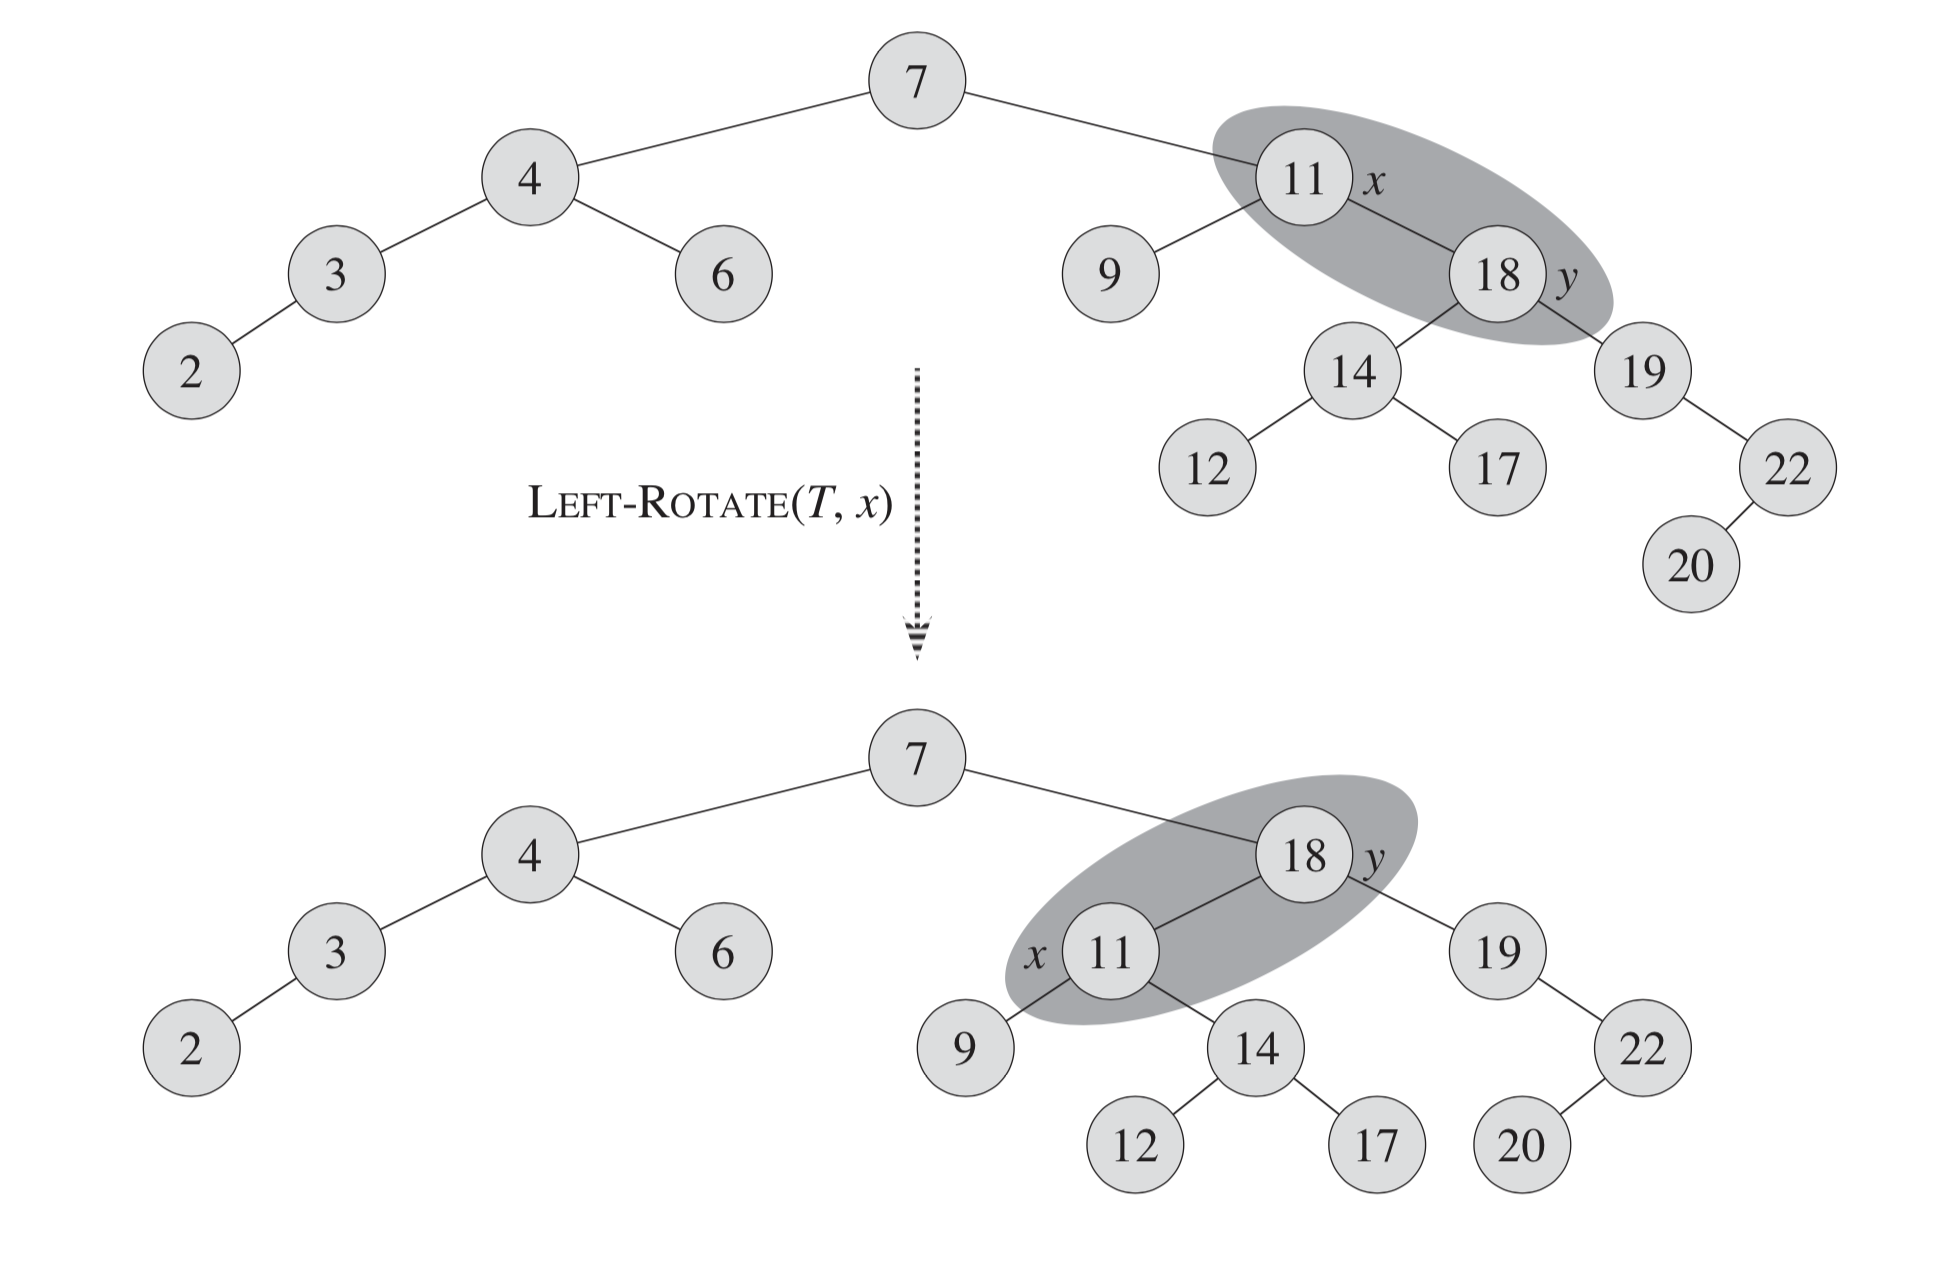
\includegraphics[scale=0.4]{rotate_ex}
\caption{
    Calling $\proc{left-rotate}$ on $x=11$, as a note, when calling $\proc{inorder-tree-walk}$ on both trees the traversals should output the same lists.
}
\label{fig: rbt3}
\end{figure}

\newpage

\section*{Insertion}
\subsection*{Simple Overview}
This is the basic process of inserting into a red-black tree.
\begin{enumerate}
    \item Perform binary search to insert $z$ and color it red.
    \item Recolor and/or rotate nodes to fix violations.
\end{enumerate}

Four cases to fix after inserting node $z$.
\begin{enumerate}
\setcounter{enumi}{-1} % start list at zero for "case 0"
    % Case 0
    \item $z$ is the root, thus, color $z$ black (we can refer to this as case 0).
    
    % Case 1
    \item $z$'s uncle is red, thus, recolor $z$'s parent, uncle, and grandparent.
    
    % figure 13.5
    \begin{figure}[!ht]
    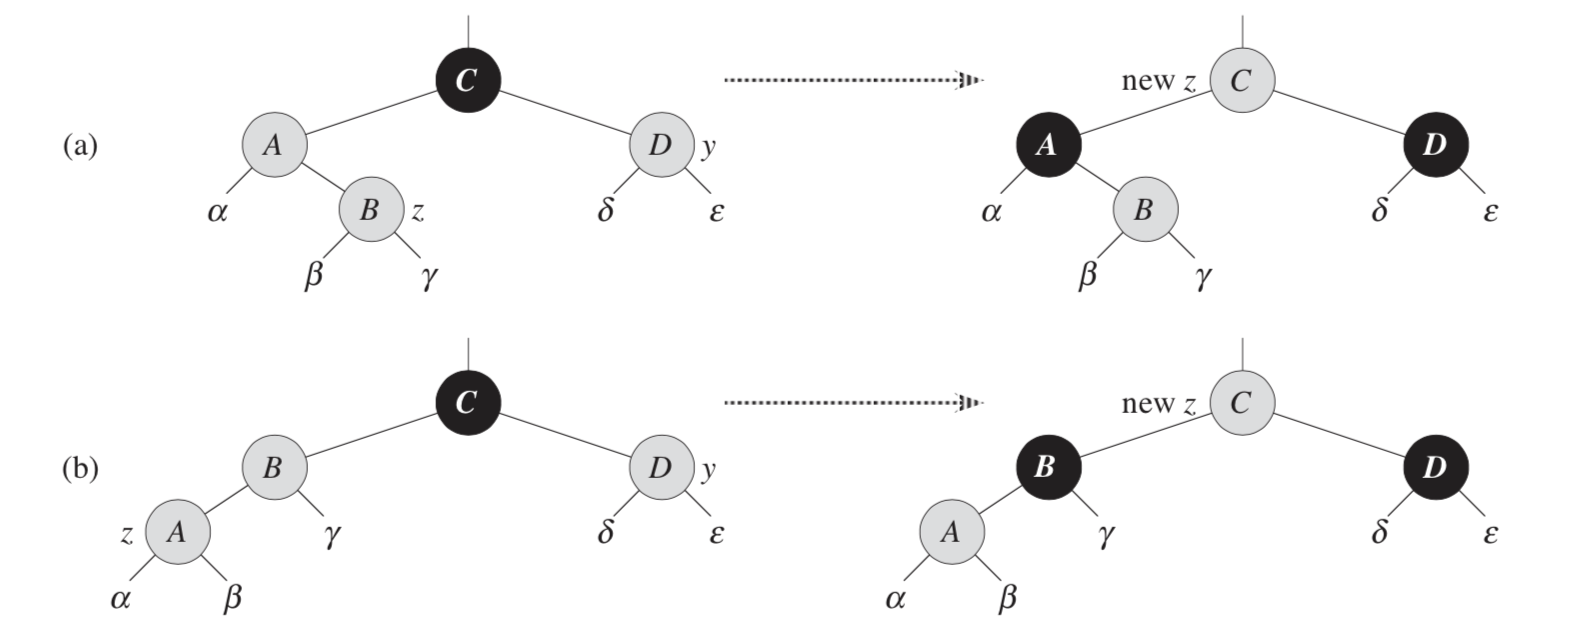
\includegraphics[scale=0.5]{rbt_insert_case1}
    \caption{
        The book's depiction of case 1. It does not matter whether $z$ is \textbf{(a)} a right child, or \textbf{(b)} a left child. Notice the black-height is preserved.
    }
    \label{fig: rbt_insert1}
    \end{figure}
    
    \begin{figure}[!ht]
    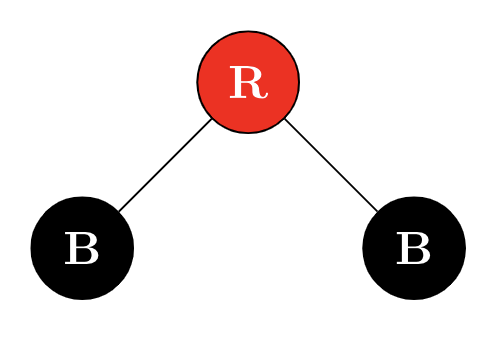
\includegraphics[scale=0.45]{rbt_insert_case1_result}
    \caption{
        The generalized result of fixing case 1. The grandfather node will always be red, while its two chilren, $z$'s parent and uncle, will be black.
    }
    \label{fig: rbt_insert2}
    \end{figure}
    
    A side-effect to this is that the grandparent (new $z$) and its parent may both be red, thus we move on to case 2.
    
    \newpage
    
    % Case 2
    \item The "triangle" case: $z$'s uncle $y$ is black and $z$, its parent, and $z$'s grandparent form a triangle-shape in the tree. We must rotate $z$'s parent in the opposite direction of $z$, so if $z$ is a right child, perform left-rotate on the parent, and vice versa. Notice no re-coloring is done, we only rotate, thus, we move on to case 3.

    % Case 3
    \item The "line" case: $z$'s uncle $y$ is black and $z$, its parent, and $z$'s grandparent form a straight line in the tree. Node $z$ and its parent are either both left or right children. To finally produce a valid red-black tree, rotate $z$'s grandparent in the opposite direction of $z$.
    
    % figure 13.6
    \begin{figure}[!ht]
    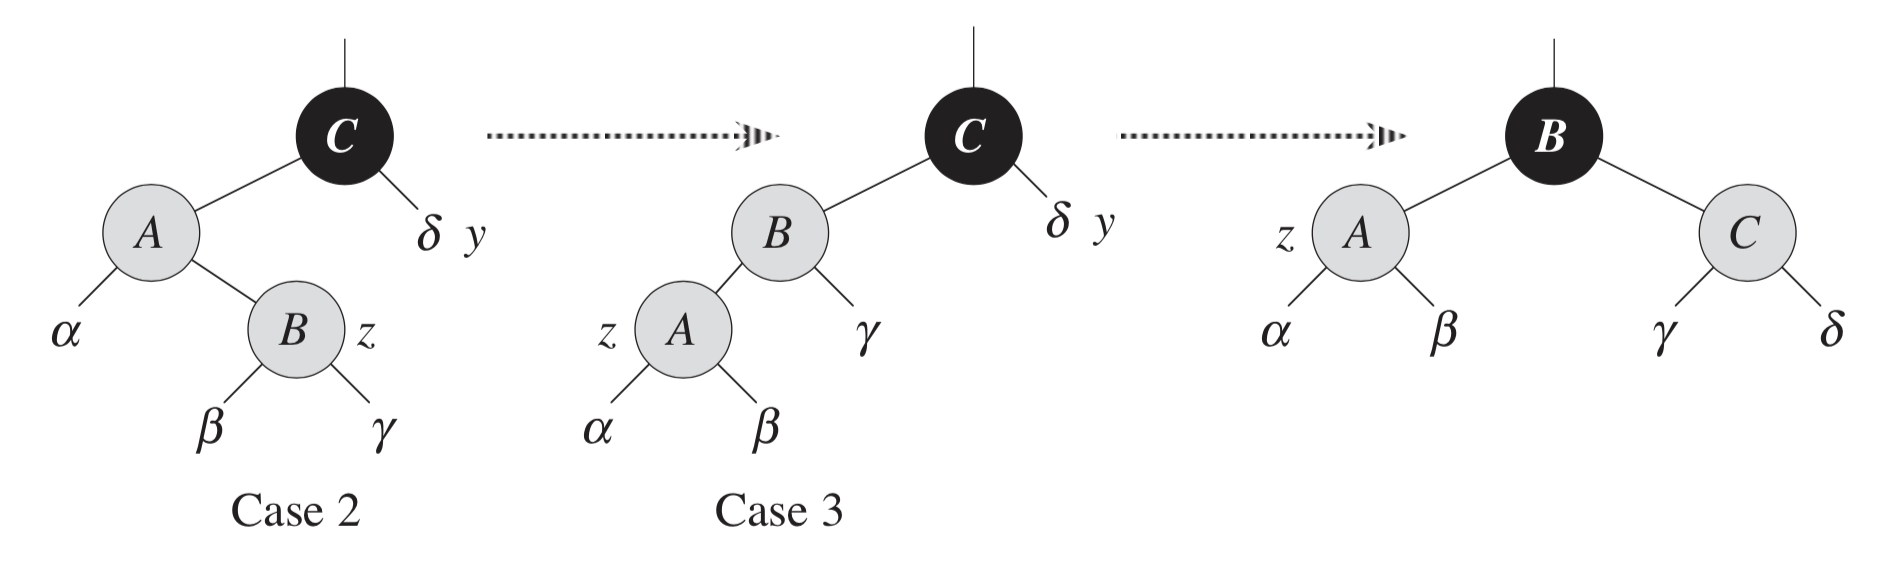
\includegraphics[scale=0.45]{rbt_insert_case2-3}
    \caption{
        Case 2 leads into case 3. $z$'s parent becomes the new root of the subtree, notice the black-height is preserved as the root is still black, we just moved red-nodes to the left and right subtrees of $z$'s parent, we now have a valid red-black tree again!
    }
    \label{fig: rbt_insert3}
    \end{figure}
    
    \begin{figure}[!ht]
    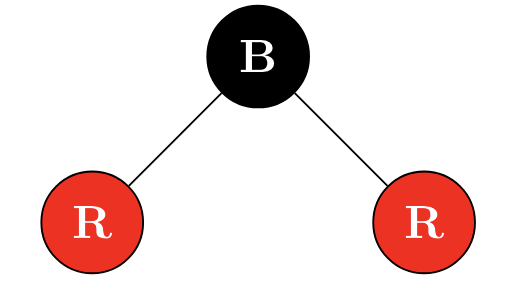
\includegraphics[scale=0.45]{rbt_insert_case2-3_result}
    \caption{
        The generalized result of fixing cases 2 and 3. Node $z$ and its grandparent are now red and children to $z$'s parent, which is now black.
    }
    \label{fig: rbt_insert4}
    \end{figure}
    
\end{enumerate}

\newpage

\subsection*{Procedures}
The procedure $\proc{rb-insert }$ adds several new lines to $\proc{tree-search}$ in order to properly insert a node into a red-black tree in $O(\log_2n)$ time. It inserts the node $z$, assigns $\attrib{T}{nil}$ to its children pointers, then assigns its color to be red, and finally calls the subroutine $\proc{rb-insert-fixup}$ to check for violations. 

%--------------------------------------------
% rb insert
%--------------------------------------------
\begin{codebox}
\Procname{$\proc{rb-insert}(T, z)$}
\li $y \gets{\attrib{T}{nil}}$
\li $x \gets{\attrib{T}{root}}$
\li \While $x \neq \attrib{T}{nil}$ \Comment perform regular binary search
    \Do
\li     $y \gets{x}$
\li     \If $\attrib{z}{key} < \attrib{x}{key}$
\li     \Then
            $x \gets{\attrib{x}{left}}$
\li     \Else
\li         $x \gets{\attrib{x}{right}}$
        \End
    \End
\li $\attrib{z}{p} \gets{y}$ \Comment make $y$ the parent, insert $z$ in the appropriate place
\li \If $y \isequal \attrib{T}{nil}$
\li \Then
        $\attrib{T}{root} \gets{z}$
\li \ElseIf $\attrib{z}{key} < \attrib{y}{key}$
\li \Then
        $\attrib{y}{left} \gets{z}$
\li \Else
\li     $\attrib{y}{right} \gets{z}$
    \End
\li $\attrib{z}{left} \gets{\attrib{T}{nil}}$
\li $\attrib{z}{right} \gets{\attrib{T}{nil}}$
\li $\attrib{z}{color} \gets{\const{red}}$
\li $\proc{rb-insert-fixup}(T, z)$
\end{codebox}

The procedure $\proc{rb-insert-fixup}$ will check if $z$'s parent is red, if so, we must then see which subtree the parent falls under, at this point solving for left or right subtrees is symmetrical. The procedure then checks which cases to fix discussed above, afterwards, the procedure calls itself on the grandparent to check if the violations have moved up the tree. Finally, the root is colored black to take care of case 0.

\newpage

%--------------------------------------------
% rb insert fixup
%--------------------------------------------
\begin{codebox}
\Procname{$\proc{rb-insert-fixup}(T, z)$}
\li \While $\attrib{z}{\attrib{p}{color} \isequal \const{red}}$
    \Do
\li     \If $\attrib{z}{p} \isequal \attrib{z}{\attrib{p}{\attrib{p}{left}}}$
\li     \Then
            $y \gets{\attrib{z}{\attrib{p}{\attrib{p}{right}}}}$
\li         \If $\attrib{y}{color} \gets{\const{red}}$ \Comment case 1
\li         \Then
                $\attrib{z}{\attrib{p}{color}} \gets{\const{black}}$
\li             $\attrib{y}{color} \gets{\const{black}}$
\li             $\attrib{z}{\attrib{p}{\attrib{p}{color}}} \gets{\const{red}}$
\li             $z \gets{\attrib{z}{\attrib{p}{p}}}$
\li         \Else
\li             \If $z \isequal \attrib{z}{\attrib{p}{right}}$ \Comment case 2
\li             \Then
                    $z \gets{\attrib{z}{p}}$
\li                 $\proc{left-rotate}(T, z)$
                \End
\li             $\attrib{z}{\attrib{p}{color}}
\gets{\const{black}}$ \Comment case 2 leads into case 3
\li             $\attrib{z}{\attrib{p}{\attrib{p}{color}}} \gets{\const{red}}$
\li             $\proc{right-rotate}(T, \attrib{z}{\attrib{p}{p}})$
            \End
% Same as then clause with "right" and "left" exchanged
\li     \Else
\li         $y \gets{\attrib{z}{\attrib{p}{\attrib{p}{left}}}}$
\li         \If $\attrib{y}{color} \gets{\const{red}}$ \Comment case 1
\li         \Then
                $\attrib{z}{\attrib{p}{color}} \gets{\const{black}}$
\li             $\attrib{y}{color} \gets{\const{black}}$
\li             $\attrib{z}{\attrib{p}{\attrib{p}{color}}} \gets{\const{red}}$
\li             $z \gets{\attrib{z}{\attrib{p}{p}}}$
\li         \Else
\li             \If $z \isequal \attrib{z}{\attrib{p}{left}}$ \Comment case 2
\li             \Then
                    $z \gets{\attrib{z}{p}}$
\li                 $\proc{right-rotate}(T, z)$
                \End
\li             $\attrib{z}{\attrib{p}{color}} \gets{\const{black}}$ \Comment case 2 leads into case 3
\li             $\attrib{z}{\attrib{p}{\attrib{p}{color}}} \gets{\const{red}}$
\li             $\proc{left-rotate}(T, \attrib{z}{\attrib{p}{p}})$
            \End
        \End
    \End
\li $\attrib{T}{\attrib{root}{black} \isequal \const{black}}$
\end{codebox}

\newpage

\section*{Deletion}
Like the other red-black procedures, deletion takes $O(\log_2n)$ time. Deletion is more complicated than regular deletion from a binary search tree, the procedure the book uses is optimized, there are other (many more) implementations that deal with \textbf{six} cases instead of four.
\\
To start, the $\proc{transplant}$ procedure needs to be modified to be used with a red-black tree. The procedure uses $\attrib{T}{nil}$ instead of $\const{nil}$, and $u$'s parent becomes $v$'s parent unconditionally.

%--------------------------------------------
% rb transplant
%--------------------------------------------
\begin{codebox}
\Procname{$\proc{rb-transplant}(T, u, v)$}
\li \If $\attrib{u}{p} \isequal \attrib{T}{nil}$
\li \Then
        $\attrib{T}{root} \gets{v}$
\li \ElseIf $u \isequal \attrib{u}{\attrib{p}{left}}$
\li \Then
        $\attrib{u}{\attrib{p}{left}} \gets{v}$
\li \Else
\li     $\attrib{u}{\attrib{p}{right}} \gets{v}$
    \End
\li $\attrib{v}{p} \gets{\attrib{u}{p}}$
\end{codebox}

The delete procedure for a red-black tree keeps track of two nodes, $y$ and $x$, that might cause violations. 

\begin{itemize}
    \item Have node $y$ point to $z$, and keep track of $y = z$'s original color.
    \item To handle the cases where $z$ has no or one child, the first two if statements on lines 3 and 6 replace $z$ with its non-nil subtree, called $x$, recall the transplant procedures take care of subtree assignment and parent pointers to and from the new node.
    \item If $z$ has two non-nil children, then reassign $y$ to be $z$'s successor by taking the minimum of the right subtree (and store the color of this successor). Node $y$ will take $z$'s place if we go into the else statement starting in line 9. Node $x$ in this case moves into $y$'s original position, and point to $y$'s right subtree.
\end{itemize}

\newpage

%--------------------------------------------
% rb delete
%--------------------------------------------
\begin{codebox}
\Procname{$\proc{rb-delete}(T, u, v)$}
\li $y \gets{z}$
\li $\id{y-original-color} \gets{\attrib{y}{color}}$
\li \If $\attrib{z}{left} \isequal \attrib{T}{nil}$
\li \Then
        $x \gets{\attrib{z}{right}}$
\li     $\proc{rb-transplant}(T, z, \attrib{z}{right})$ \Comment replace $z$ with right non-nil subtree
\li \ElseIf $\attrib{z}{right} \isequal \attrib{T}{nil}$
\li \Then
        $x \gets{\attrib{z}{left}}$
\li     $\proc{rb-transplant}(T, z, \attrib{z}{left})$ \Comment replace $z$ with left non-nil subtree
\li \Else
\li     $y \gets{\proc{tree-minimum}(\attrib{z}{right})}$
\li     $\id{y-original-color} \gets{\attrib{y}{color}}$
\li     $x \gets{\attrib{y}{right}}$
\li     \If $\attrib{y}{p} \isequal z$
\li     \Then
            $\attrib{x}{p} \gets{y}$
\li     \Else
            $\proc{rb-transplant}(T, y, \attrib{y}{right})$
\li         $\attrib{y}{right} \gets{\attrib{z}{right}}$
\li         $\attrib{y}{\attrib{right}{p}} \gets{y}$
        \End
\li     $\proc{rb-transplant}(T, z, y)$
\li     $\attrib{y}{left} \gets{\attrib{z}{left}}$
\li     $\attrib{y}{\attrib{left}{p}} \gets{y}$
\li     $\attrib{y}{color} \gets{\attrib{z}{color}}$
    \End
\li \If $\id{y-original-color} \isequal \const{black}$
\li \Then
        $\proc{rb-delete-fixup}(T, x)$
    \End
\end{codebox}

If node $y$ was red (the node we moved to replace $z$), we are done. The black-height did not change. No red nodes are adjacent because $y$ takes on $z$'s color; if $y$ was not $z$'s right child, $y$'s right child $x$ that replaces it has to be black, we essentially removed a red node from one path in the tree, which does not damage the red-black height property. Since $y$ could not have been the root, the root remains black.
\\
If in these steps, node $y$ was black, we may have violated one or more red-black properties, thus the call to $\proc{rb-delete-fixup}$. According to the book, these are the potential causes:

\begin{itemize}
    \item If $y$ had been the root and a red child of $y$ becomes the new root, we have violated property 2.
    \item If both $x$ and $\attrib{x}{p}$ are red, then we have violated property 4.
    \item Moving $y$ within the tree causes any simple path that previously contained $y$ to have one fewer black node. Thus, property 5 is now violated by any ancestor of $y$ in the tree.
\end{itemize}

To fix the violation of property 5, the idea of a ``\textbf{double black}'' node is introduced. We must essentially move the double black to another node and perform rotations to move this to a satisfactory spot. The procedure $\proc{rb-delete-fixup}$ fixes this issue, it focuses on $x$, recall it replaced $y$, which replaced $z$.

%--------------------------------------------
% rb delete fixup
%--------------------------------------------
\begin{codebox}
\Procname{$\proc{rb-delete-fixup}(T, u, v)$}
\li \While $x \neq \attrib{T}{root}$ and $\attrib{x}{color} \isequal \const{black}$
\li \Do
        \If $x \isequal \attrib{x}{\attrib{p}{left}}$
\li     \Then
            $w \gets{\attrib{x}{\attrib{p}{right}}}$
\li         \If $\attrib{w}{color} \isequal \const{red}$ \Comment case 1 in then clause
\li         \Then
                $\attrib{w}{color} \gets{\const{black}}$
\li             $\attrib{x}{\attrib{p}{color}} \gets{red }$
\li             $\proc{left-rotate}(T, \attrib{x}{p})$
\li             $w \gets{\attrib{x}{\attrib{p}{right}}}$
            \End
\li         \If $\attrib{w}{\attrib{left}{color}} \isequal \const{black}$ and $\attrib{w}{\attrib{right}{color}} \isequal \const{black}$ \Comment case 2
\li         \Then
                $\attrib{w}{color} \gets{red}$
\li             $x \gets{\attrib{x}{p}}$
\li         \Else
\li             \If $\attrib{w}{\attrib{right}{color}} \isequal \const{black}$ \Comment case 3
\li             \Then
                    $\attrib{w}{\attrib{left}{color}} \gets{\const{black}}$
\li                 $\attrib{w}{color} \gets{red}$
\li                 $\proc{right-rotate}(T, w)$
\li                 $w \gets{\attrib{x}{\attrib{p}{right}}}$
                \End
\li             $\attrib{w}{color} \gets{\attrib{x}{\attrib{p}{color}}}$ \Comment case 4
\li             $\attrib{x}{\attrib{p}{color}} \gets{\const{black}}$
\li             $\attrib{w}{\attrib{right}{color}} \gets{\const{black}}$
\li             $\proc{left-rotate}(T, \attrib{x}{p})$
\li             $x \gets{\attrib{T}{root}}$
            \End
% same as then clause with "right" and "left" exchanged
\li     \Else
\li         $w \gets{\attrib{x}{\attrib{p}{left}}}$
\li         \If $\attrib{w}{color} \isequal \const{red}$ \Comment case 1 in then clause
\li         \Then
                $\attrib{w}{color} \gets{\const{black}}$
\li             $\attrib{x}{\attrib{p}{color}} \gets{red }$
\li             $\proc{right-rotate}(T, \attrib{x}{p})$
\li             $w \gets{\attrib{x}{\attrib{p}{left}}}$
            \End
\li         \If $\attrib{w}{\attrib{right}{color}} \isequal \const{black}$ and $\attrib{w}{\attrib{left}{color}} \isequal \const{black}$ \Comment case 2
\li         \Then
                $\attrib{w}{color} \gets{red}$
\li             $x \gets{\attrib{x}{p}}$
\li         \Else
\li             \If $\attrib{w}{\attrib{left}{color}} \isequal \const{black}$ \Comment case 3
\li             \Then
                    $\attrib{w}{\attrib{right}{color}} \gets{\const{black}}$
\li                 $\attrib{w}{color} \gets{red}$
\li                 $\proc{left-rotate}(T, w)$
\li                 $w \gets{\attrib{x}{\attrib{p}{left}}}$
                \End
\li             $\attrib{w}{color} \gets{\attrib{x}{\attrib{p}{color}}}$ \Comment case 4
\li             $\attrib{x}{\attrib{p}{color}} \gets{\const{black}}$
\li             $\attrib{w}{\attrib{left}{color}} \gets{\const{black}}$
\li             $\proc{right-rotate}(T, \attrib{x}{p})$
\li             $x \gets{\attrib{T}{root}}$
            \End
        \End
    \End
\li $\attrib{x}{color} \gets{\const{black}}$
\end{codebox}

\newpage
Looking at the procedure $\proc{rb-insert-fixup}$, $x$ always points to a nonroot doubly black node. Next, determine if $x$ is a left or right child (either case is symmetrical, just switch ``left'' and ``right''). The pointer $w$ refers to $x$'s sibling, note that $w$ cannot be $\attrib{T}{nil}$ as the black-height from $\attrib{x}{p}$ to $x$ and to $w$ must be the same. In each of the four cases $\proc{rb-insert-fixup}$ fixes, property 5 must be preserved after each transformation executed on the \textit{subtrees} rooted at $x$ and $w$.
\\ \\
\textbf{Case 1: $x$'s sibling $w$ is red}\\
Since $w$ is red, its children must be black, thus we switch the colors of $\attrib{x}{p}$ and $w$, and then perform a left rotation on $\attrib{x}{p}$. Node $x$'s new sibling, previously one of $w$'s children, is now black. \textbf{\emph{Move on to case 2, 3, or 4}}.
\\ \\
Cases 2, 3, and 4 occur when node $w$ is black, they are distinguished by the colors of $w$'s children.
\\ \\
\textbf{Case 2: $x$'s sibling $w$ is black, and both of $w$'s children are black}\\
We take one black from both $x$ and $w$, and put it on $\attrib{x}{p}$ (which could be red or black). Next, treat $\attrib{x}{p}$ as the new $x$, and keep going up the red-black tree. This is how we recolor nodes red to adjust the black-height, thus satisfying property 5. \textbf{\emph{Stop, we are done}}!
\\ \\
\textbf{Case 3: $x$'s sibling $w$ is black, $w$'s left child is red, and and $w$'s right child is black}\\
Switch the colors of $w$ and $\attrib{w}{left}$, and then right-rotate on $w$. Node $x$'s new sibling $w$ is black with a red right child.
\textbf{\emph{Move on to case 4}}.
\\ \\
\textbf{Case 4: $x$'s sibling $w$ is black, and $w$'s right child is red}\\
This case makes several color changes (look at the procedure), and then left-rotate on $\attrib{x}{p}$. Doing so allows $w$ to remove the extra black on $x$ without any violations. Setting $x$ as the root satisfies the first condition for the while loop and the red-black tree is finally fixed. \textbf{\emph{Stop, we are done}}!

\subsection*{Analysis}
With a red-black tree with $n$ nodes having a height of $O(\log_{2}n)$, only deleting takes $O(\log_{2}n)$ time. In $\proc{rb-delete-fixup}$, cases 1, 3, and 4 only take constant time, case 2 is the only case where the while loop repeats going up the tree at most $O(\log_{2}n)$ times. Thus $\proc{rb-delete-fixup}$ takes $O(\log_{2}n)$.

\newpage

% figure 13.7
\begin{figure}[!ht]
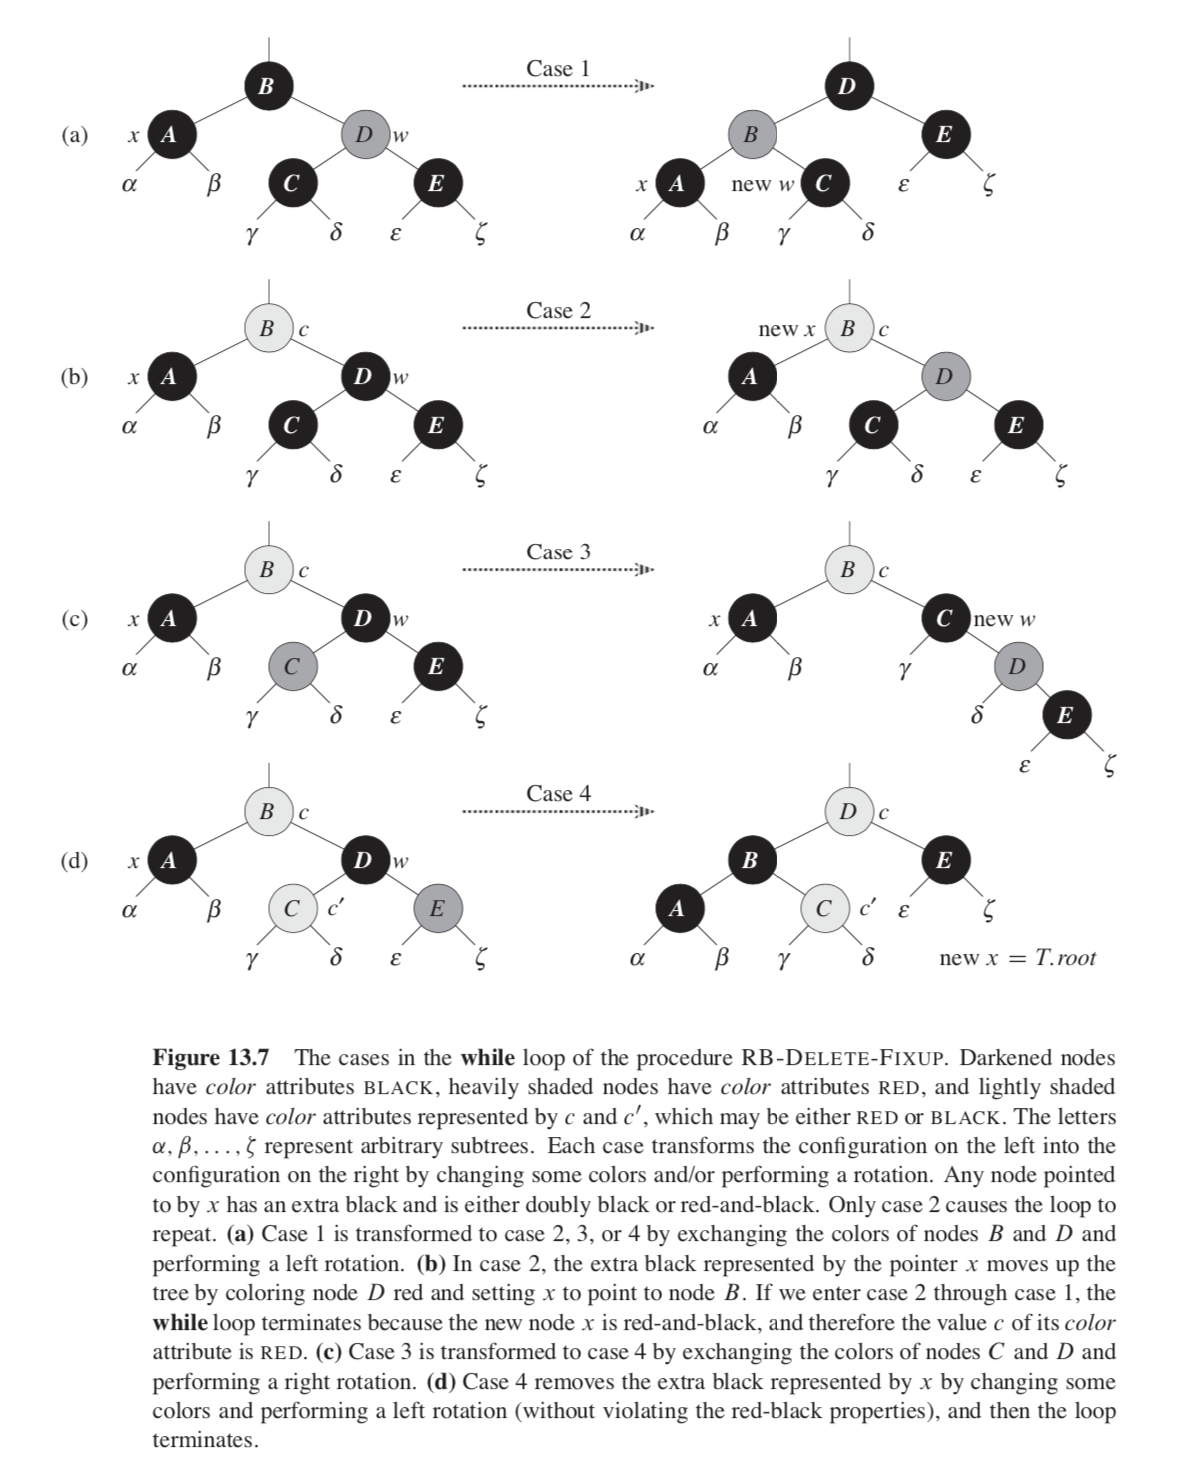
\includegraphics[scale=0.7]{rbt_delete}
\label{fig: rbt_delete}
\end{figure}

\end{document}
